%%%%%%%%%%%%%%%%%%%%%%%%%%%%%%%%%%%%%%%%%%%%%%%%%%%%%%%%%%%%%%%%%%%%%%%%%%%%%
%
%  System        : 
%  Module        : 
%  Object Name   : $RCSfile$
%  Revision      : $Revision$
%  Date          : $Date$
%  Author        : $Author$
%  Created By    : Robert Heller
%  Created       : Mon Jul 15 17:33:37 2019
%  Last Modified : <190717.1702>
%
%  Description 
%
%  Notes
%
%  History
% 
%%%%%%%%%%%%%%%%%%%%%%%%%%%%%%%%%%%%%%%%%%%%%%%%%%%%%%%%%%%%%%%%%%%%%%%%%%%%%
%
%    Copyright (C) 2019  Robert Heller D/B/A Deepwoods Software
%			51 Locke Hill Road
%			Wendell, MA 01379-9728
%
%    This program is free software; you can redistribute it and/or modify
%    it under the terms of the GNU General Public License as published by
%    the Free Software Foundation; either version 2 of the License, or
%    (at your option) any later version.
%
%    This program is distributed in the hope that it will be useful,
%    but WITHOUT ANY WARRANTY; without even the implied warranty of
%    MERCHANTABILITY or FITNESS FOR A PARTICULAR PURPOSE.  See the
%    GNU General Public License for more details.
%
%    You should have received a copy of the GNU General Public License
%    along with this program; if not, write to the Free Software
%    Foundation, Inc., 675 Mass Ave, Cambridge, MA 02139, USA.
%
% 
%
%%%%%%%%%%%%%%%%%%%%%%%%%%%%%%%%%%%%%%%%%%%%%%%%%%%%%%%%%%%%%%%%%%%%%%%%%%%%%

\chapter{QuadSMCSenseHat: Quad Motor Control and Sense HAT}

This is a circuit board to for an add-on board for a Raspberry Pi B+ that will
control four stall-motor turnout motors for a model railroad. It also has
sense logic to return the state of the turnouts, using one pole of the DPDT
contacts in the stall-motor (typical of Tortoise stall-motors).

The circuit board uses a 40pin header socket to connect to the 40pin header on
the  Raspberry Pi B+ and can use a  stack-through  header to allow  additional
boards to be stacked on top of it.

\section{GPIO Pins Used and stacking restrictions.}

This board uses eight GPIO pins:

\begin{description}
\item[WiringPi 0, BCM 17] Motor Select 1: select the position of stall motor 
1. 
\item[WiringPi 1, BCM 18] Motor Select 2: select the position of stall motor 
2. 
\item[WiringPi 2, BCM 27] Point Sense 1: return the state of the points for 
stall motor 1. 
\item[WiringPi 3, BCM 22] Point Sense 2: return the state of the points for 
stall motor 2. 
\item[WiringPi 4, BCM 23] Motor Select 3: select the position of stall motor 
3. 
\item[WiringPi 5, BCM 24] Motor Select 4: select the position of stall motor 
4. 
\item[WiringPi 6, BCM 25] Point Sense 3: return the state of the points for 
stall motor 3. 
\item[WiringPi 7, BCM 4] Point Sense 4: return the state of the points for 
stall motor 4. 
\end{description}

Each of the motor drive circuits is through a TC4428, which can drive up to
1.5A, which is way more needed to drive typical stall motor. It is enough to
drive a pair of stall motors, wired in parallel as would be the case for a
cross over. 

Because this board is hardwired to use eight specific GPIO pins it is not 
possible to use two or more of these boards on given Raspberry Pi.

\section{Circuit Description}

\begin{figure}[hbpt]\begin{centering}%
\includegraphics[width=5in]{QuadSMCSenseHat.pdf}
\caption{Circuit Diagram of the QuadSMCSenseHat}
\end{centering}\end{figure}
This circuit contains two sections.  There is an output section that contains 
four TC4428 chips.  Each chip has a non-inverting and an inverting driver. The 
inputs of both drivers are connected to one of the motor GPIO pins.  The 
output are wired to the terminal block for a one of the motors. For any given 
logic state of the motor control output, one of the drivers is ``on'' and the 
other is ``off'', thus one motor terminal is ground and one is raised to the 
12V supply.  This means alternative states of the logic line will drive the 
stall motor in alternative directions.

The other section is a quartet of flip-flop debounce circuits, one for each
of two SPDT switch contacts that report the position of the turnout points.
The output of these flip-flops goes to a quartet of GPIO input pins.

\section{Parts List}

\begin{table}[htdp]
\begin{centering}\begin{tabular}{|l|l|p{1in}|l|p{.5in}|}
\hline
Value&Quantity&References&Mouser Part Number&Adafruit Part Number \\
\hline
.1 uf&2&C1 C2&581-SR201C104KARTR1& \\
\hline
10 uf 35V&1&C3&667-ECA-1HM100I& \\
\hline
RPi\_GPIO&1&J0&855-M20-6102045& \\
\hline
10K Ohms&1&RR1&652-4609X-1LF-10K& \\
\hline
Motor 1;Motor 2;Motor 3;Motor 4&4&T1 T2 T3 T4&651-1725685& \\
\hline
+ 12V -&1&T5&651-1725656& \\
\hline
TC4428&4&U1 U2 U3 U4&579-TC4428VPA& \\
\hline
74HCT00&2&U5 U6&595-SN74AHC00N& \\
\hline
\end{tabular}
\caption{Parts list for QuadSMCSenseHat board.}
\end{centering}\end{table}\footnote{Mouser Project link: 
\url{http://www.mouser.com/ProjectManager/ProjectDetail.aspx?AccessID=330542c522}.}


The only parts that might be substituted are J0 (the RPi GPIO Header), and T1 
though T4 (the Motor terminals) and T5 (the 12 to 16 Volts terminals).  The parts 
listed are for the stacking headers for the RPi GPIO Header, and screw 
terminals for the Motor terminals and the motor power terminals.  Feel free to 
select a non-stacking header for the RPi GPIO Header and to select either pin 
arrays or spring terminals for the T1, T2, T3, T4 and T5.

\section{Circuit Board Layout}

\begin{figure}[hbpt]\begin{centering}%
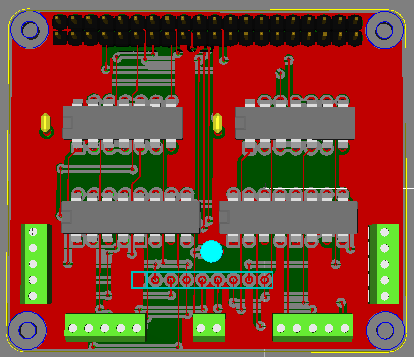
\includegraphics[width=5in]{QuadSMCSenseHat3DTop.png}
\caption{3D rendering of the QuadSMCSenseHAT board}
\end{centering}\end{figure}
\begin{figure}[hbpt]\begin{centering}%
\includegraphics[width=5in]{QuadSMCSenseHat.png}
\caption{Fabrication image of the QuadSMCSenseHAT board}
\end{centering}\end{figure}
Board assembly is straight forward. You need to be careful orienting the ICs
and the electrolytic capacitor.

Bare circuit boards can be ordered from PCBWay here: 
\url{https://www.pcbway.com/project/shareproject/Quad_Stall_Motor_Controller_w__point_Sense__hat_.html}.

\section{Downloadables and Software Support}

Full design information is available on GitHub here:
\url{https://github.com/RobertPHeller/RPi-RRCircuits/tree/master/QuadSMCSenseHat}.

An OpenMRN program that supports this board is available here:
\url{https://github.com/RobertPHeller/RPi-RRCircuits/tree/master/QuadSMCSenseOpenMRN}.
This board is also supported by the Model Railroad System\footnote{Available
as a free download from Deepwoods Software at this web address:
\url{http://www.deepsoft.com/home/products/modelrailroadsystem/}.}
\texttt{OpenLCB\_PiGPIO} daemon. A basic XML file for it is included in its
GitHub folder.


